\chapter{Revisão Bibliográfica} \label{cap:rev}

\section{Fundamentação teórica} 

Várias empresas aproveitam a crescente acessibilidade da população a dispositivos móveis, criando suas aplicações e disponibilizando seus produtos em lojas virtuais como Apple Store e Play Store, respectivamente lojas da plataforma IOS e Android.
Muitas destas empresas criaram seus impérios utilizando-se de frotas de entregadores e fornecedores sem ter a necessidade de gastar com veículo ou produto, apenas gerenciando seus colaboradores. Como exemplos, temos o caso do Uber: empresa voltada a transporte pessoal similar ao sistema de Táxi; Airbnb: uma empresa voltada a gerenciar locais para pousadas, hotelarias ou aluguel residencial sem ter seu próprio local de atuação; Ifood: um dos grandes nomes de entrega de comidas existentes sem ter seu restaurante próprio.
O projeto proposto foi baseado em demanda de mercado existente e projetos correlatos no exterior para auxiliar nas etapas de desenvolvimento e ajudar na interpretação dos dados adquiridos e na própria execução do projeto. Esta parte do documento tem como objetivo mostrar os benefícios que estes novos aplicativos geram para a sociedade além de seus riscos.

\subsection{Mercado em crescimento}
De acordo com a notícia escrita por COSTA (2019), do jornal O Globo, o setor de transporte gerou 133 mil vagas em fevereiro graças a utilização dos aplicativos móveis, pois basta você ter um veículo para se locomover e ser apto a realizar entregas. Segundo os dados adquiridos pelo autor através da Confederação Nacional do Comércio ou CNC entre os anos de 2008 e 2018 houve um crescimento de 74\% somente no número de motociclistas no Rio de Janeiro. 

\subsection{Riscos}

Segundo BOM DIA SP (2019), a quantidade de acidentes fatais ocorridos por motociclistas aumentou 17,7\% em 2018 relação a 2017 na cidade de São Paulo, chegando a uma média de pelo menos uma morte por dia. Destaca-se, também, o fato de que os aplicativos de entregas dão bônus em dinheiro para aqueles que fazem mais entregas em menor espaço de tempo.
Outra notícia é do Estadão de São Paulo que cita o aumento de aproximadamente 18\% de acidentes com motociclistas com uma influência em aplicativos, a matéria possui um mapa contendo todos os pontos de acidentes ocorridos em 2017 e 2018, mostrado na Figura 2.1. (RIBEIRO e FELIX, 2019)


\begin{figure}[H]

 \caption{Mapa contendo todos os pontos de mortes registradas por motociclistas}
  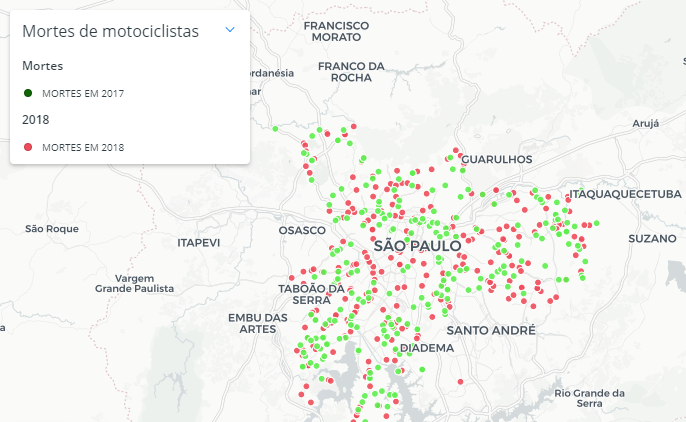
\includegraphics[width=\textwidth]{images/Cap2/mapa.png}
  
  
\end{figure}


Também é destacado o estímulo exagerado por estes aplicativos de entregas que incentivam os motociclistas a saírem para realizar suas entregas mesmo em condições desfavoráveis, oferecendo uma comissão por realizar suas entregas como é demonstrado na Figura 2.2, que contém mensagens de SMS de alguns aplicativos de delivery conhecidos atualmente.


\begin{figure}[H]

 \caption{Mensagens de incentivos recebidas por motociclistas}
  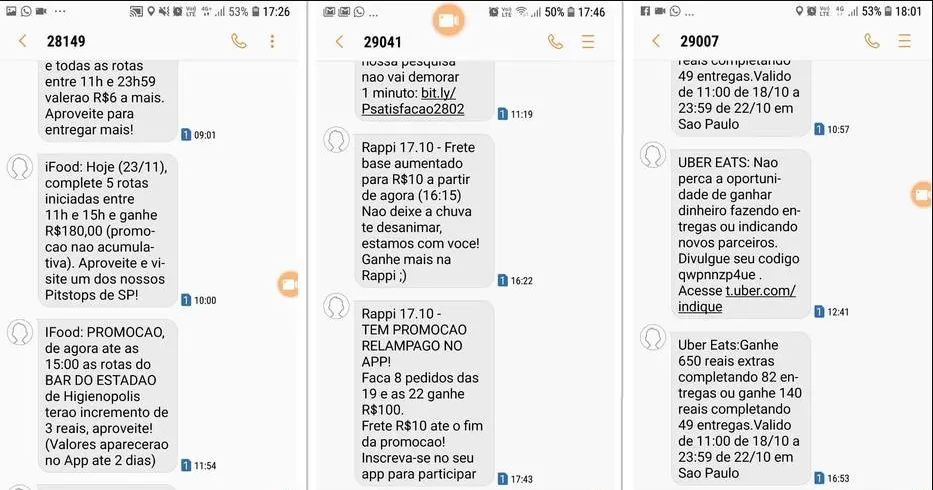
\includegraphics[width=\textwidth]{images/Cap2/whtas.png}
  
\end{figure}


\section{Trabalhos correlatos}

2.2.1 Estudo da dinâmica das motocicletas em frenagens e curvas: O efeito da técnica do piloto e da condição da estrada

Como Magnani e Cunha (2017) demonstram em seu estudo sobre a dinâmica das motocicletas em frenagens e curvas, a técnica do piloto nas mais adversas situações é determinante para manter-se sob controle em situações de risco. Nesse estudo objetivaram determinar a velocidade máxima para a realização de curvas determinadas e quando o piloto deve iniciar a frenagem a fim de evitar acidentes. 
O estudo envolveu a análise de diversas forças que atuam sobre o veículo, como demonstradas na Figura 2.3.


\subsection{Estudo da dinâmica das motocicletas em frenagens e curvas: O efeito da técnica do piloto e da condição da estrada}

Como Magnani e Cunha (2017) demonstram em seu estudo sobre a dinâmica das motocicletas em frenagens e curvas, a técnica do piloto nas mais adversas situações é determinante para manter-se sob controle em situações de risco. Nesse estudo objetivaram determinar a velocidade máxima para a realização de curvas determinadas e quando o piloto deve iniciar a frenagem a fim de evitar acidentes. 
O estudo envolveu a análise de diversas forças que atuam sobre o veículo, como demonstradas na Figura 2.3.
    
\begin{figure}[H]

 \caption{Forças existentes no movimento e frenagem da motocicleta}
 \centering
  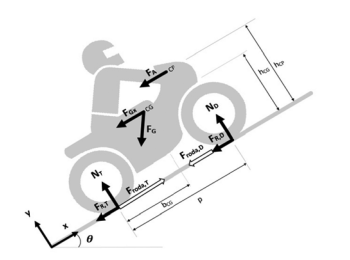
\includegraphics[width=150mm]{images/Cap2/forca.png}
  \end{figure}
  
\clearpage




Neste estudo se destacam as informações de ângulo, taxa e força de desaceleração máximas de certos eventos, de forma a auxiliar no reconhecimento de possíveis acidentes. 

Em sua conclusão, os autores identificaram que a desaceleração é altamente dependente do coeficiente de atrito em cada situação, de forma a não recomendar uma técnica universal de frenagem. Todos os cenários estudados foram elevados ao limite onde, com exceção de pilotos profissionais, raramente é atingido cotidianamente.


\subsection{Monitoramento da agressividade na direção de caminhões}

O trabalho publicado por Schlag (2017) utiliza um sistema embarcado composto por um microcontrolador, acelerômetro, GPS e GSM para monitorar as ações dos motoristas de caminhões, determinando se o comportamento ao dirigir é perigoso e sinalizando tal comportamento por e-mail. Os dados obtidos pelo sistema embarcado são enviados para um servidor que compila e mostra a trajetória do motorista, bem como os trechos nos quais houve agressividade em sua condução como demonstra a Figura 2.4.


\begin{figure}[H]

 \caption{Forças existentes no movimento e frenagem da motocicleta}
 \centering
  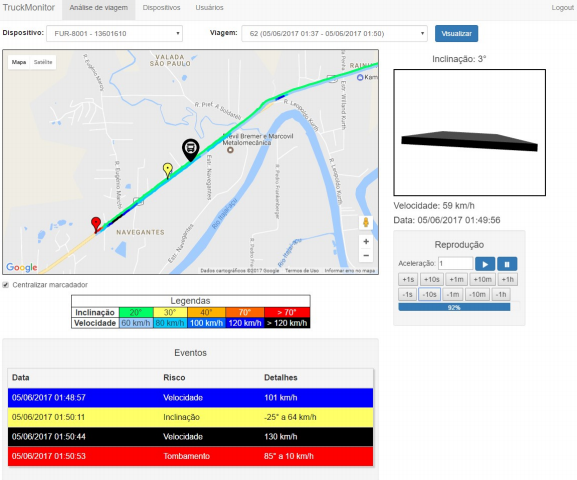
\includegraphics[width=100mm]{images/Cap2/analise.png}
  
\end{figure}

Neste trabalho, o autor obteve grande assertividade ao detectar excessos de velocidade, conseguindo aferir a mesma com precisão de 4 km/h. Tombamentos e possíveis manobras perigosas também foram registrados. Inclusive as manobras agressivas realizadas para evitar acidentes, nesses casos o dispositivo foi movimentado manualmente a fim de evitar manobras arriscadas. 



\subsection{Proposta de emprego de giroscópio e acelerômetro na perícia de acidentes automobilísticos}

No artigo publicado na Revista Brasileira de Criminalística, Lima e Ricardo (2017), propuseram um dispositivo embarcado de baixo custo capaz de registrar os dados em acidentes de carro. Em países desenvolvidos, o módulo do sistema de air bag também coleta os dados que resultaram em sua ativação. Citando a literatura internacional, os autores buscam algo semelhante à “caixa preta” que é, ou deveria ser no caso de veículos nacionais, o módulo de air bag. 

Motivados pelo difícil acesso aos scanners exclusivos dos fabricantes dos veículos e/ou módulos de air bag, buscaram capturar e analisar os dados de segundos antes e após o acidente, de forma a auxiliar no estudo criminalístico. 

Utilizando um sistema embarcado dotado de acelerômetro e giroscópio, o dispositivo foi capaz de armazenar 10,9 segundos de informações relacionadas ao acidente. Tais informações podem ser exportadas para simuladores 3D capazes de reconstruir virtualmente o acidente, em sua conclusão reforçam a grande aplicabilidade de seu sistema, auxiliando os peritos e experts no assunto. 


\subsection{Uso de Smartphones para monitoramento de ciclistas e detecção automática de acidentes}


O projeto proposto pelos alunos da universidade tecnológica de Chalmers é alertar acidentes de ciclistas utilizando o eCall.

eCall é um sistema desenvolvido na Europa capaz de monitorar os veículos na estrada, na ocorrência de alguns acidentes o dispositivo acoplado no veículo faz uma ligação para o número de emergência, além de passar as coordenadas do veículo para as autoridades. (EUROPEAN COMMISSION, 2019)

Como o sistema de eCall é voltado somente para automóveis foi proposto pelos alunos da universidade de Chalmers na Suécia implementar o sistema de eCall utilizando smartphones para ciclistas, como demonstrado na Figura 6.  Neste projeto não foi utilizado nenhum hardware adicional para a medição dos dados, o smartphone não precisou de nenhuma fonte de energia externa, pois o aplicativo desenvolvido era econômico em relação a drenagem da bateria do celular.



\begin{figure}[H]

 \caption{Princípio do funcionamento do sistema de eCall para ciclista}
 \centering
  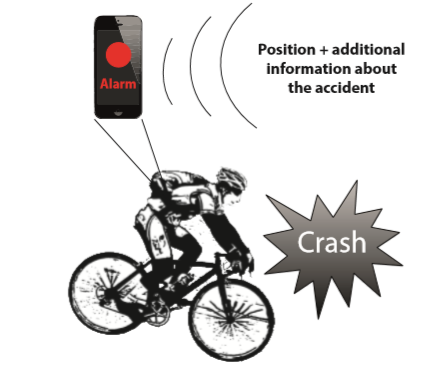
\includegraphics[width=150mm]{images/Cap2/images.png}
  
\end{figure}


Para o monitoramento foram utilizados os seguintes sensores para a medição dos dados, acelerômetro de 3 eixos, sensor de rotação de 3 eixos e sensor de posição GPS com uma taxa de amostragem de 100hz, todos eles já integrados dentro do smartphones. Com isto foi possível calcular a aceleração total do ciclista utilizando a equação (2.1)

\begin{equation}
\centering
    \mathit{Acc} = \sqrt{Accx^2 + Accy^2 + Accz^2}
\end{equation}


Para a aquisição dos dados foram registradas mais de 5 horas de dados “normais” onde nenhum acidente ocorreu. Já para os registros de impacto foi utilizado um boneco, que possui as características humanas e um peso de 40kg, que foi submetido a vários testes de queda.

 O Gráfico da Figura 2.6 demonstra uma amostra dos dados coletados. O primeiro intervalo, entre zero e quarenta segundos, representa o ajuste do celular em cima da bicicleta, já o intervalo de noventa e cem segundos mostra um padrão de indicação de acidente.

\begin{figure}[H]

 \caption{Gráfico dos dados mensuradas}
  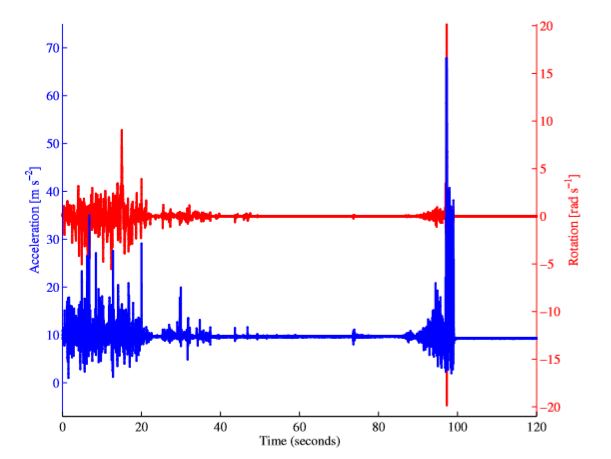
\includegraphics[width=150mm]{images/Cap2/grafico_acelera.png}
    
\end{figure}

Estudando este projeto, foi possível concluir que é possível utilizar somente um smartphone para a detecção de uma queda ou acidente, sendo possível disparar sinais de emergência para outros lugares.

\subsection{Utilizando smartphones com sensor móvel sem fio para a detecção de acidentes de carro e providenciar avisos de emergências}

No artigo de Thompson et al. (2010) foi proposto o desenvolvimento de um aplicativo para smartphone responsável por capturar os dados dos sensores de acelerômetro, compasso e GPS, sendo capaz de detectar acidentes e gravar estes dados, como a força G exercida no usuário durante o evento.

O sistema foi desenvolvido no formato cliente-Servidor, o smartphone envia as informações via internet móvel para o servidor utilizando HTTP post, onde os dados recebidos serão processados e, então, enviará notificações para as autoridades. Na Figura 2.7 é apresentado o esquemático do sistema criado.

\begin{figure}[H]

 \caption{Sistema de detecção de acidentes}
  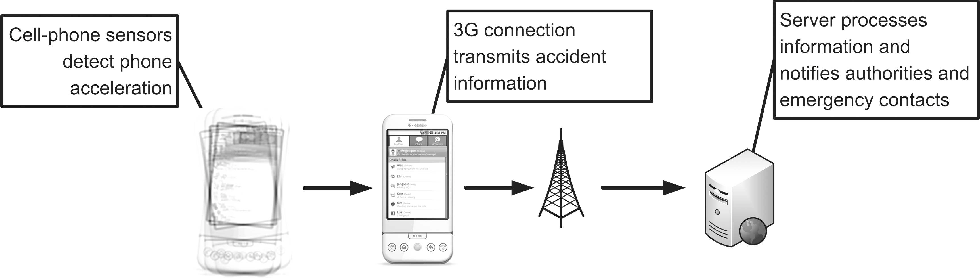
\includegraphics[width=150mm]{images/Cap2/esquema.png}
  
    
\end{figure}


O sistema irá monitorar o comportamento do acelerômetro de três eixos do celular, quando houver uma grande aceleração pelos ocupantes será registrada a força aplicada em relação ao usuário, registrando um evento contendo o valor da força G e a posição do ocorrido, a Figura 2.8 demonstra quando o aplicativo é acionado.


\begin{figure}[H]

 \caption{Sistema de detecção de acidentes}
  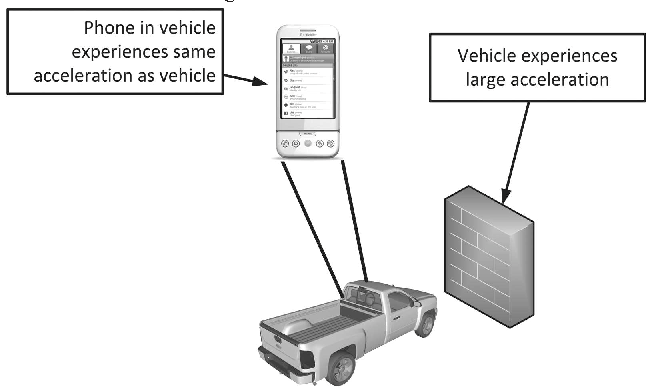
\includegraphics[width=150mm]{images/Cap2/acionamento.png}
  
    
\end{figure}


Porém ainda foi necessário verificar os casos falso positivo e removê-los do sistema para que não tenha avisos errados pelo sistema, para isto foram analisados dois casos:

\begin{itemize}
    \item  Filtro de velocidade que determina onde o usuário está no veículo
    
    Para prevenir problemas de arranque o aplicativo só começa a medir um potencial acidente a partir de 24 km/h, além disso o sistema fica ativo por 5 minutos mesmo após a desaceleração do veículo, fazendo com que o aplicativo não tenha que ficar recriando sua conexão toda vez que o usuário pare em um semáforo.
\end{itemize}


\begin{itemize}
    \item  Filtro de aceleração que previne paradas bruscas para o acionamento das notificações.
    
    Para isto o sistema irá ignorar qualquer aceleração bruta menos do que 4G, para isto foram feitos dois testes para determinar estes efeitos, o primeiro foi acelerar o carro até 38 km/h e frear bruscamente gerando o resultado da Figura 2.9.
    
\end{itemize}


\begin{figure}[H]

 \caption{Gráfico mostrando os efeitos dos 3 eixos a parada brusca}
  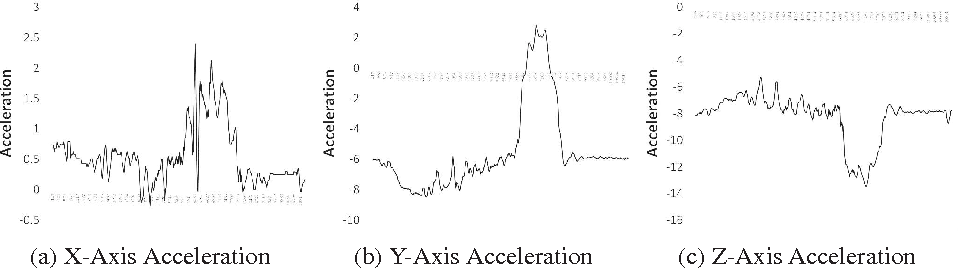
\includegraphics[width=150mm]{images/Cap2/acelerometro_graficos.png}
  
    
\end{figure}


O segundo teste foi deixar o celular cair em queda livre e verificar os valores do acelerômetro, determinando então que a variação dos acelerômetros foram apenas picos de energia muito rápido registrados como mostra a Figura 2.10.



\begin{figure}[H]

 \caption{Gráfico mostrando os 3 eixos do acelerômetro para a queda livre}
  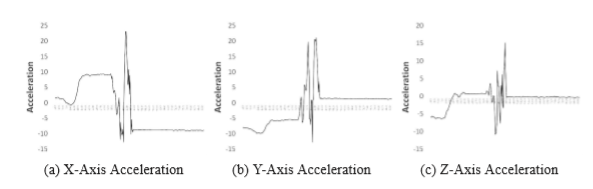
\includegraphics[width=150mm]{images/Cap2/acelerometro_quedalivre.png}
  \end{figure}
Com este projeto foi possível concluir que é viável utilizar um smartphone que transmita as informações para um servidor externo pois há uma redução do custo do desenvolvimento e manutenção do serviço, além de não ser necessário a aquisição de um hardware específico.
